\chapter{Anàlisi i disseny del sistema}

L'anàlisi i disseny del sistema s'explicarà des dels components més petits fins als més grans, amb un diagrama per a cadascun al final dels seus respectius apartats.

\section{Servidor Local}

El nostre servidor s'executa en forma de contenidor juntament amb \textit{Redis}, una base de dades que corre a memòria volàtil (RAM), que també s'executa en forma de contenidor. El Docker Engine s'encarrega que els ports dels contenidors s'exposin a la màquina amfitriona com si estiguessin executant-se directament en ella, en un procés conegut com a publicació de ports \cite{noauthor_publishing_0100}. Això vol dir que quan la màquina amfitriona consulta el port 8085, que és el que s'assigna per defecte a la imatge de \textit{clue-api} per a la màquina amfitriona, Docker Engine redirigeix aquesta consulta al port corresponent del contenidor, i de la mateixa manera, redirigeix la resposta de tornada a l'equip amfitrió.

Per altra banda, també s'executa de manera nativa l'aplicació Netdata per tal de publicar, com a webapp, les anàlisis dels recursos del portàtil.

Posteriorment, el tallafocs esmentat al \autoref{cap:9} permet el trànsit de peticions als ports que hem escollit des de la xarxa local externa a la màquina i bloqueja els altres per raons de seguretat. Finalment, el nostre rúter + NAT, que té la IP única a internet, s'encarrega de redirigir els paquets entrants pels ports que escollim deixar oberts a internet cap a una màquina específica de la xarxa local, que en aquest cas és la Màquina-Servidor.

\begin{figure}[!htbp] 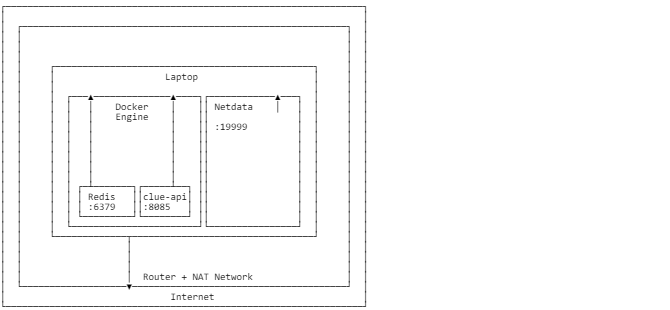
\includegraphics[width=1.75\textwidth]{Imatges/Server-Local.png} \label{fig:ServerLocal
} \caption{Diagrama de l'arquitectura del servidor local} \end{figure}

\newpage
\section{Servidor al Núvol}
L'arquitectura del servidor al núvol és molt similar a la del servidor local, amb la diferència que la nostra màquina e2-micro es troba en una xarxa compartida amb altres instàncies de màquines anomenada \textit{default}. L'obertura de ports per a permetre l'accés des d'internet a la màquina es realitza a nivell de les \textit{VPC}, que són les xarxes virtuals que ofereix Google per a les màquines al núvol.\cite{noauthor_vpc_nodate}

\begin{figure}[!htbp] 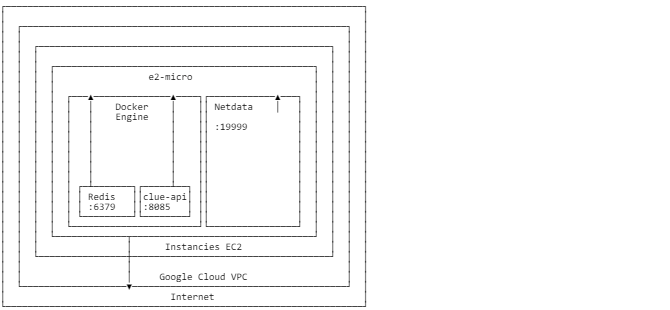
\includegraphics[width=1.75\textwidth]{Imatges/Server-Cloud.png} \label{fig:ServerNuvul
} \caption{Diagrama de l'arquitectura del servidor al núvol} \end{figure}
    

\newpage

\section{Client}

Pel que fa al client, aquest comença amb l'script de k6, on es creen dinàmicament els Virtual Users, que són fils molt lleugers anomenats \textit{Goroutines}. Cada un d'aquests fils, que simula un usuari, genera peticions específiques a la xarxa de manera constant, des del seu naixement fins a la seva mort, de manera seqüencial, però amb execució concurrent entre tots els usuaris virtuals. Cadascuna d'aquestes crides es realitza directament a internet a través del rúter, sense necessitat de gestionar cap redirecció de ports, ja que la connexió és iniciada per l'ordinador i, per tant, queda registrada automàticament.\cite{stoykov_why_nodate}

\begin{figure}[!htbp] 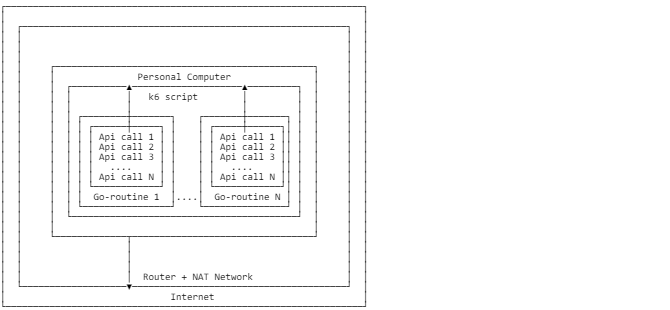
\includegraphics[width=1.75\textwidth]{Imatges/Client-Local.png}  \label{fig:ClientLocal} \caption{Diagrama de l'arquitectura del client} \end{figure}

